\section{Data retrieval}

  The purpose of this thesis was to analyse the discussions that may appear on message boards (or Internet forums) or news groups, hence a set of data like that had to be obtained. I had a freedom of choice, so I decided to take a look at the messages posted on an Internet forum called \emph{head-fi} (http://www.head-fi.org/f/). It is a forum gathering users wanting to talk about audio equipment such as headphones (mainly), amplifiers or speakers. I was already familiar with this message board so I knew---\textit{more or less}---what to expect from the community taking part in conversations on this forum. I also knew the \emph{physical} topological structure so it was easier for me to write the software used to \emph{crawl} the site and save the messages in my database.
  
  Initially, I have anticipated to download every single message posted on this forum from the beginning of its existence and that was neither hidden nor removed---i.e. available to browse---at the time of downloading the data. I looked at the most recent \emph{identifier} (or ID) of a post and knew that the total number of messages posted on the forum was nearing $8.5$ million, providing that the posts were not removed during its existence. Section \ref{sec:crawling} describes procedures used to browse the forum.
  
  \subsection{Data structure}
    Because the messages on the Internet forums are traditionally saved in a relational dabatase I have decided to reflect the structure of this particular forum in my own---also relational---database, but with a simpler, more fit to my needs, structure.
    
    I chose to split the board into three logical parts: \emph{forums}, \emph{topics} (or \emph{threads}) and \emph{posts} (or \emph{messages}) that were also following the order in which the message board was being crawled. Because posts are written by \emph{users} (or \emph{members}), I have also decided to further \emph{normalise} the database by creating a separate table for them. The structure of the database at a time was then as presented in tables \ref{tab:data_forums}, \ref{tab:data_topics}, \ref{tab:data_users} and \ref{tab:data_posts}, containing all the information I could---and wanted---to save.
    \begin{table}[H]
      \begin{tabularx}{\textwidth}{|L{0.3}|L{1.7}|} \hline
        \rowcolor[gray]{0.75} \textbf{Field} & \textbf{Description} \\\hline
        id & Unique identifier; referenced in topics table as forum\_id. \\
        title & The title of the forum as text. \\\hline
      \end{tabularx}
      \caption{Forums table structure.}
      \label{tab:data_forums}
    \end{table}
    
    \begin{table}[H]
      \begin{tabularx}{\textwidth}{|L{0.3}|L{1.7}|} \hline
        \rowcolor[gray]{0.75} \textbf{Field} & \textbf{Description} \\\hline
        id & Unique identifier; referenced in posts table as topic\_id. \\
        forum\_id & Reference of a forum, the topic is in. \\
        title & The title of the topic as text. \\\hline
      \end{tabularx}
      \caption{Topics table structure.}
      \label{tab:data_topics}
    \end{table}
    
    \begin{table}[H]
      \begin{tabularx}{\textwidth}{|L{0.3}|L{1.7}|} \hline
        \rowcolor[gray]{0.75} \textbf{Field} & \textbf{Description} \\\hline
        id & Unique identifier; referenced in posts table as user\_id. \\
        name & The name of the user as text. \\\hline
      \end{tabularx}
      \caption{Users table structure.}
      \label{tab:data_users}
    \end{table}
    
    \begin{table}[H]
      \begin{tabularx}{\textwidth}{|L{0.3}|L{1.7}|} \hline
        \rowcolor[gray]{0.75} \textbf{Field} & \textbf{Description} \\\hline
        id & Unique identifier. \\
        in\_reply\_to & A comma separated list of IDs of the posts that were quoted in this post. \\
        topic\_id & ID of the topic the post is in. \\
        user\_id & ID of the user that is the author of this post. \\
        date & Date and time the message was posted. \\
        body & Post contents as text. \\\hline
      \end{tabularx}
      \caption{Posts table structure.}
      \label{tab:data_posts}
    \end{table}
    
    A database table with posts features a \emph{in\_reply\_to} field which I thought would be good to have to specifically bind messages that quote others. However, it was never used later.
    
  \subsection{Web crawling}
    \label{sec:crawling}
    
      Starting out from the Home Page I had to download the list of forums first. Algorithm \ref{alg:crawl_forums_list} shows the procedure needed to do that. After running it I had 25 sub-forums available to crawl deeper into the message board.
  
    \begin{algorithm}[H]
      \begin{algorithmic}[1]
        \Procedure{CrawlForumsList}{url}
          \State html $\gets$ \textsc{FetchUrl}(url)
          \State anchors $\gets$ \textsc{ForumTitleAnchors}(html)
          \ForAll{anchor \textbf{in} anchors}
            \State forumId $\gets$ \textsc{IdFromAnchor}(anchor)
            \State forumTitle $\gets$ \textsc{TitleFromAnchor}(anchor)
            \State \textsc{WriteToDB}(``Forums'', forumId, forumTitle)
          \EndFor
        \EndProcedure
      \end{algorithmic}
      \caption{Crawl forums list.}
      \label{alg:crawl_forums_list}
    \end{algorithm}
    
    Then I started with \emph{Headphones (full-size)} forum (the first one on the list) and I began crawling this forum and fetching the topics. This task was a little more complicated, because the topics were not listed all on one page. Instead, they were paginated\footnote{\emph{Pagination} is a process of dividing the content into discrete chunks, called pages. It is used mostly to limit the number of results displayed to the user in order to both reduce the amount of data the server is required to send and the client is required to receive.}: 50 topics per page. I have decided not to use \emph{brute force} techniques to crawl the topics list, but to approach the problem more intelligently and simulate web browser along with HTML parser that allowed me to find and follow hyperlinks labelled as \textquote{Next page}. Procedure required to accomplish this task is featured in the listing of algorithm \ref{alg:crawl_forums}.
  
    \begin{algorithm}[H]
      \begin{algorithmic}[1]
        \Procedure{CrawlForums}{forumUrlFormat}
          \State forums = \textsc{ReadFromDB}(``Forums'') \Comment{Set of (forumId, forumTitle) tuples from DB}
          \ForAll{(forumId, forumTitle) \textbf{in} forums}
            \State nextUrl $\gets$ \textsc{PrepareUrl}(forumUrlFormat, forumId)
            \Repeat
              \State html $\gets$ \textsc{FetchUrl}(nextUrl)
              \State anchors $\gets$ \textsc{TopicTitleAnchors}(html)
              \ForAll{anchor \textbf{in} anchors}
                \State topicId $\gets$ \textsc{IdFromAnchor}(anchor)
                \State topicTitle $\gets$ \textsc{TitleFromAnchor}(anchor)
                \State \textsc{WriteToDB}(``Topics'', topicId, topicTitle, forumId)
              \EndFor
              \State nextUrl $\gets$ \textsc{NextUrl}(html) \Comment{Taken from \textquote{Next} hyperlink}
            \Until nextUrl \textbf{is not} $\varnothing$
          \EndFor
        \EndProcedure
      \end{algorithmic}
      \caption{Crawl forums.}
      \label{alg:crawl_forums}
    \end{algorithm}
    
    One problem arose during the fetching of post threads: \emph{bumping}. Bumping is a phenomenon occurring on virtually every message board that have time assigned to each posted message. When a member of the forum posts in a thread it will jump to the top of the list since it is the latest updated thread. That meant that after all pages have been crawled, I had to repeatedly crawl the beginning of the list until I found no new topics on the first page of the sub-forum to save to database.
    
    Last step involved browsing the threads in order to save individual messages. It was very similar to the previous one because posts were also paginated. However, this time, bumping was not a problem, since messages inside threads were ordered by time they were posted in ascending order (first-come, first-served), so I only need to crawl each topic once. The process is shown as an algorithm \ref{alg:crawl_topics} below.
  
    \begin{algorithm}[H]
      \begin{algorithmic}[1]
        \Procedure{CrawlTopics}{topicUrlFormat}
          \State topics = \textsc{ReadFromDB}(``Topics'') \Comment{Set of (topicId, topicTitle) tuples from DB}
          \ForAll{(topicId, topicTitle) \textbf{in} topics}
            \State nextUrl $\gets$ \textsc{PrepareURL}(topicUrlFormat, topicId)
            \Repeat
              \State html $\gets$ \textsc{FetchUrl}(nextUrl)
              \State posts $\gets$ \textsc{Posts}(html)
              \ForAll{post \textbf{in} posts}
                \State postId $\gets$ \textsc{IdFromPost}(post)
                \State postBody $\gets$ \textsc{BodyFromPost}(post)
                \State postDate $\gets$ \textsc{DateFromPost}(post)
                \State userId $\gets$ \textsc{UserFromPost}(post)
                \State quotes $\gets$ \textsc{QuotedFromPost}(post)
                \State \textsc{WriteToDB}(``Posts'', postId, postBody, postDate, userId, quotes, topicId)
              \EndFor
              \State nextUrl $\gets$ \textsc{NextUrl}(html) \Comment{Taken from \textquote{Next} button}
            \Until nextUrl \textbf{is not} $\varnothing$
          \EndFor
        \EndProcedure
      \end{algorithmic}
      \caption{Crawl topics.}
      \label{alg:crawl_topics}
    \end{algorithm}
    
    Executing the three crawling procedures mentioned above took a long time for a single sub-forum so I have decided to stop further browsing. I had a lot of data to analyse so it was not crucial to continue. Table \ref{tab:data_count} displays the number of entities in the database I have extracted.
    
    \begin{table}[H]
      \centering
      \begin{tabularx}{0.5\textwidth}{|L{1}|R{1}|} \hline
        \rowcolor[gray]{0.75} \textbf{Entity} & \textbf{Total count} \\\hline
        Forums & $25$ \\\hline
        Topics & $111,047$ \\\hline
        Posts & $1,941,970$ \\\hline
        Users & $52,605$ \\\hline
      \end{tabularx}
      \caption{Total count of extracted entities.}
      \label{tab:data_count}
    \end{table}
    
    At this point, I had one type of nodes that would form my bipartite network: users. Now it was time to get the other type---words---but they had to be extracted first, which I describe in the following section.
    
  \subsection{Word extraction}

    Words had to be extracted from the post message, excluding any quotations from earlier posts as they would pollute the actual word usage by users. The process was divided into three parts: \emph{text segmentation}, \emph{word classification} and \emph{word stemming}.
    
    \subsubsection{Text segmentation} \label{sec:text_segmentation}
    
      Fortunately, the problem of hyphenation, where words are split by syllables for presentation purposes (in justified text, especially in articles and books) and then conjoined with hyphens is non-existent in Internet forums due to the fact that advanced text rendering (like hyphenation) is not yet supported in widely used web browsers.

      After several iterations of trial and error I have finally decided to segment words using a regular expression. The final pattern was: \texttt{/\textbackslash s+|-\{2,\}|(?!-)\textbackslash p\{P\}+/}. It consists of three subpatterns that try to segment words in three ways. The breakdown of this pattern can be found in table \ref{tab:splitpattern}. The \textquote{\texttt{|}} (also called \emph{pipe}) character denotes an \texttt{OR} statement inside this regular expression meaning that any one of the subpatterns provided cause the word to split.
      
      \begin{table}[H]
        \begin{tabularx}{\textwidth}{|L{0.3}|L{1.7}|} \hline
          \rowcolor[gray]{0.75} \textbf{Pattern} & \textbf{Description} \\\hline
          \textbackslash s+ & One or more whitespace characters. \\
          -\{2,\} & Two or more hyphens. \\
          (?!-)\textbackslash p\{P\}+ & One or more punctuation characters not preceded by a hyphen, without matching said hyphen. It will split when two or more hyphens are encountered or at least one other punctuation character. \\\hline
        \end{tabularx}
        \caption{Breakdown of splitting regular expression pattern.}
        \label{tab:splitpattern}
      \end{table}
      
      I thought it will be interesting to check whether the number of new distinct words that appeared during segmentation conform to the Heaps' law, which formulated as $V_R(n) = Kn^\beta$ has parameter $K$ typically between $10$ and $100$, and parameter $\beta$ typically between $0.4$ and $0.6$ in english texts. In figure \ref{fig:word_extraction} the red crosses represent the actual numbers (on axis $OX$) of words after the number of posts (on axis $OY$) where blue line is the function $V_R(n)$ that has been fitted to that set of numbers with the values of parameters $K = 83.3 \pm1.1 (1.313\%)$ and $\beta = 0.5984 \pm0.0009 (0.1557\%)$ respectively. 
      
      \begin{figure}[H]
        \centering
        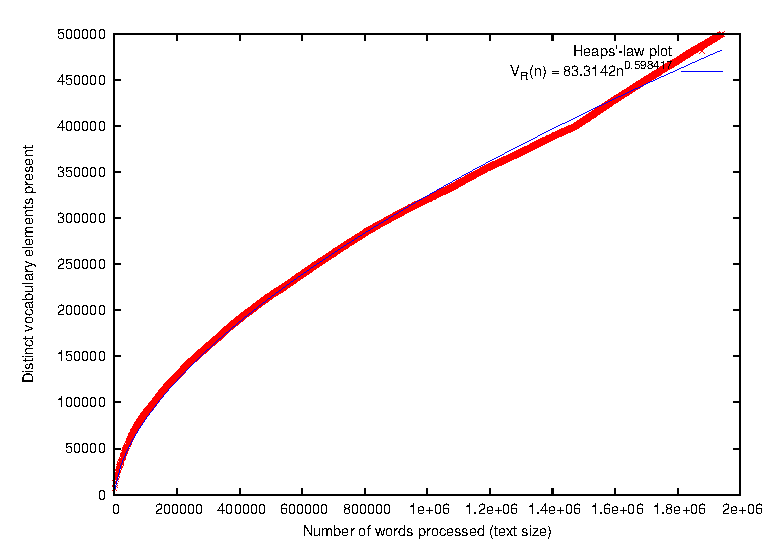
\includegraphics[width=\textwidth]{chapters/03_implementation/extraction}
        \caption{Heaps'-law plot in linear scale.}
        \label{fig:word_extraction}
      \end{figure}
      
      This is a perfect indication that the messages posted by the users of the head-fi forum I am analysing conform to Heaps' law. Figure \ref{fig:word_extraction_log} shows the same in logarythmic scale.
      
      \begin{figure}[H]
        \centering
        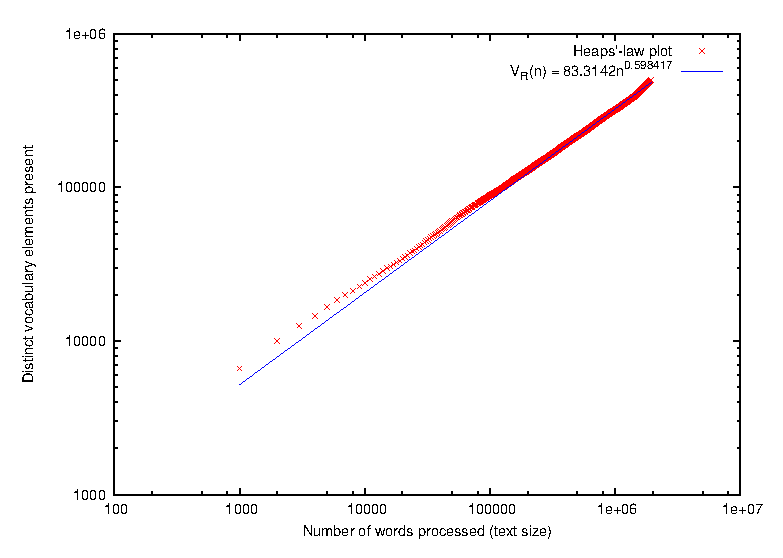
\includegraphics[width=\textwidth]{chapters/03_implementation/extraction_log}
        \caption{Heaps'-law plot in logarithmic scale.}
        \label{fig:word_extraction_log}
      \end{figure}


    \subsubsection{Word classification}
    
      The three main groups of words I have selected to use are \emph{products}, \emph{opinions} and \emph{prices}. Words that did not fit into one of these were not classified, i.e. left as just regular words.
    
      \paragraph{Products}
      
        To create a list of keywords identifying products (and brands) I had to browse a lot of music equipment related websites and create a list by parsing menus, categories and other text on these pages. I have also used price comparison services which were a great help since I could browse to \emph{headphones} category and download a list of products of which prices they compared.
        
        A list of brands and products was then manually checked for correctness and the entries that seemed too generic, like \emph{audio}, \emph{sound} or \emph{bass} were removed. After all that I ended having 4,500 keywords related to products.
      
      \paragraph{Opinions}
      
        Opinions were divided into \emph{positive} and \emph{negative}. Examples of both sub-groups can be found in tables \ref{tab:positiveopinionsexamples} and \ref{tab:negativeopinionsexamples}.
        
        \begin{table}[H]
          \begin{subtable}{0.49\textwidth}
            \centering
            \begin{tabularx}{0.75\textwidth}{|L{1}|L{1}|} \hline
              \rowcolor[gray]{0.8} \textbf{Positive opinion} \\\hline
              love \\
              portable \\
              convincing \\
              recommend \\
              nice \\
              superb \\
              neat \\
              comfortable \\
              beautiful \\
              incredible \\
              \hline
            \end{tabularx}
            \caption{Selected examples of positive opinions.}
            \label{tab:positiveopinionsexamples}
          \end{subtable}
          \begin{subtable}{0.49\textwidth}
            \centering
            \begin{tabularx}{0.75\textwidth}{|L{1}|L{1}|} \hline
              \rowcolor[gray]{0.8} \textbf{Negative opinion} \\\hline
              joke \\
              laugh \\
              distracting \\
              lacking \\
              incompetent \\
              bad \\
              boring \\
              suspicious \\
              horrid \\
              terrible \\
              \hline
            \end{tabularx}
            \caption{Selected examples of negative opinions.}
            \label{tab:negativeopinionsexamples}
          \end{subtable}
          \caption{Selected examples of opinions.}
          \label{tab:opinionsexamples}
        \end{table}

      \paragraph{Prices}
      
        Prices were very easy to classify. As the forum is used mostly by \emph{Americans}\footnote{Inhabitants of the United States of America} and \emph{Canadians} the price is usually denoted as \$$x$, USD$x$ or CAD$x$, where \$, USD and CAD are a currency marks and $x$ is the actual price (in various formats, but that does not matter).

    \subsubsection{Word stemming}
    
      After words have been split and classified, it turned out that there exist some discrepancies in \textquote{conventions} used by users to discuss the products.
      
      The first part of the process involved normalisation of found words. This had to be done due to problems in finding \emph{the} right word splitting pattern. Some words were prefixed or suffixed by additional characters that were not correct.
      
      Because the forum is using English language exclusively and the results of stemming non-keyword words are not critical I have decided to use non-aggressive suffix-stripping algorithm. I was not interested in finding correct root of a word, because a generic stem would be sufficient. Stems were then interpolated into root words that were being used the most.
      
      What was not covered here were typographical errors that could not easily be corrected in an automated way and the effort of manual intervention would not be justified and using automatic correction according to English dictionary could be too risky.
      \\\\
      Separate problem was finding stems for products. Many headphone models differ only by a prefix or suffix letter(s). Additionally, users tend to refer to many models appending a \emph{s} letter to the model name. For example, one user wrote \textquote{I ruined my grado SR80s.} while discussing \emph{Grado SR80} headphone model. The problem is that some models have this \textquote{extra} \emph{s} letter appended to the model name itself, example being \emph{Denon AH-NC732s} headphones. This meant that while stemming keywords related to products U had to be \emph{extremely} cautious and careful---any error here would skew the results later.
      
      Fortunately, I had a solid base of products gathered from classification step that made this process somewhat easier, as I could almost automatically remove unnecesary \emph{s} by marking the products that did not have it in their name. The product keyword number was reduced to 3,668 (23\% reduction) thanks to that process.
      
    \subsubsection{Results} \label{sec:cs_results}

      The resulting word set I could begin to work with is presented in table \ref{tab:words}. Keywords represent $4.38\%$ of all words.
      \begin{table}[H]
        \centering
        \begin{tabularx}{\textwidth}{|L{1}|L{1}|L{1}|L{1}|L{1}|L{1}|L{1}|} \hline
          \rowcolor[gray]{0.8} \textbf{Products} & \textbf{Positive opinions} & \textbf{Negative opinions} & \textbf{Prices} & \textbf{Function words} & \textbf{Regular words} & \textbf{Total words} \\\hline
$3,668$ & $2,111$ & $4,360$ & $10,259$ & $1,085$ & $468,532$ & $490,015$\footnotemark \\\hline
        \end{tabularx}
        \caption{Breakdown of the number of words and the category they belong to.}
        \label{tab:words}
      \end{table}
      \footnotetext{The number certainly looks very high but there are over 2 billion words contained in Oxford English Corpus\cite{OxfordEnglishCorpus}}
      
      The results were saved into separate database table for further reference and usage. Its structure is shown in table \ref{tab:db_relationships}. I have decided to call this table a \emph{relationship} table, because it indicates clear associations between the words written by users as posts.
      \begin{table}[H]
        \begin{tabularx}{\textwidth}{|L{0.3}|L{1.7}|} \hline
          \rowcolor[gray]{0.75} \textbf{Field} & \textbf{Description} \\\hline
          user\_id & Unique user reference; found in users table as id. \\
          word\_id & Unique word reference; found in words table as id. \\
          post\_id & Unique post reference; found in posts table as id. \\
          used & Date the word has been used; equal to post data. \\
          meta & Metadata indicating the type of keyword if necessary. \\\hline
        \end{tabularx}
        \caption{Relationships table structure.}
        \label{tab:db_relationships}
      \end{table}
